% Options for packages loaded elsewhere
\PassOptionsToPackage{unicode}{hyperref}
\PassOptionsToPackage{hyphens}{url}
%
\documentclass[
  12pt,
]{article}
\usepackage{lmodern}
\usepackage{amssymb,amsmath}
\usepackage{ifxetex,ifluatex}
\ifnum 0\ifxetex 1\fi\ifluatex 1\fi=0 % if pdftex
  \usepackage[T1]{fontenc}
  \usepackage[utf8]{inputenc}
  \usepackage{textcomp} % provide euro and other symbols
\else % if luatex or xetex
  \usepackage{unicode-math}
  \defaultfontfeatures{Scale=MatchLowercase}
  \defaultfontfeatures[\rmfamily]{Ligatures=TeX,Scale=1}
  \setmainfont[]{Times New Roman}
\fi
% Use upquote if available, for straight quotes in verbatim environments
\IfFileExists{upquote.sty}{\usepackage{upquote}}{}
\IfFileExists{microtype.sty}{% use microtype if available
  \usepackage[]{microtype}
  \UseMicrotypeSet[protrusion]{basicmath} % disable protrusion for tt fonts
}{}
\makeatletter
\@ifundefined{KOMAClassName}{% if non-KOMA class
  \IfFileExists{parskip.sty}{%
    \usepackage{parskip}
  }{% else
    \setlength{\parindent}{0pt}
    \setlength{\parskip}{6pt plus 2pt minus 1pt}}
}{% if KOMA class
  \KOMAoptions{parskip=half}}
\makeatother
\usepackage{xcolor}
\IfFileExists{xurl.sty}{\usepackage{xurl}}{} % add URL line breaks if available
\IfFileExists{bookmark.sty}{\usepackage{bookmark}}{\usepackage{hyperref}}
\hypersetup{
  pdftitle={White Salmon River Pre and Post Dam Removal},
  pdfauthor={Kristine Swann},
  hidelinks,
  pdfcreator={LaTeX via pandoc}}
\urlstyle{same} % disable monospaced font for URLs
\usepackage[margin=2.54cm]{geometry}
\usepackage{longtable,booktabs}
% Correct order of tables after \paragraph or \subparagraph
\usepackage{etoolbox}
\makeatletter
\patchcmd\longtable{\par}{\if@noskipsec\mbox{}\fi\par}{}{}
\makeatother
% Allow footnotes in longtable head/foot
\IfFileExists{footnotehyper.sty}{\usepackage{footnotehyper}}{\usepackage{footnote}}
\makesavenoteenv{longtable}
\usepackage{graphicx,grffile}
\makeatletter
\def\maxwidth{\ifdim\Gin@nat@width>\linewidth\linewidth\else\Gin@nat@width\fi}
\def\maxheight{\ifdim\Gin@nat@height>\textheight\textheight\else\Gin@nat@height\fi}
\makeatother
% Scale images if necessary, so that they will not overflow the page
% margins by default, and it is still possible to overwrite the defaults
% using explicit options in \includegraphics[width, height, ...]{}
\setkeys{Gin}{width=\maxwidth,height=\maxheight,keepaspectratio}
% Set default figure placement to htbp
\makeatletter
\def\fps@figure{htbp}
\makeatother
\setlength{\emergencystretch}{3em} % prevent overfull lines
\providecommand{\tightlist}{%
  \setlength{\itemsep}{0pt}\setlength{\parskip}{0pt}}
\setcounter{secnumdepth}{5}

\title{White Salmon River Pre and Post Dam Removal}
\usepackage{etoolbox}
\makeatletter
\providecommand{\subtitle}[1]{% add subtitle to \maketitle
  \apptocmd{\@title}{\par {\large #1 \par}}{}{}
}
\makeatother
\subtitle{\url{https://github.com/kmswann/WhiteSalmon.git}}
\author{Kristine Swann}
\date{}

\begin{document}
\maketitle

\newpage
\tableofcontents 
\newpage
\listoftables 
\newpage
\listoffigures 
\newpage

\hypertarget{rationale-and-research-questions}{%
\section{Rationale and Research
Questions}\label{rationale-and-research-questions}}

The White Salmon River (White Salmon) is a tributary of the Columbia
River in Southern Washington. It provides habitat for at least 5
threatened and endangered fish species and is one of the best white
water rivers in the US (Pesanti, 2016). In 1913, a hydroelectric dam,
the Condit Dam, was built 3 miles from the mouth of the river (Figure 1:
White Salmon River). The dam acted as barrier to salmon species and also
to kayakers who paddle both upper reaches of the river and a short
section below the dam.

Below hydroelectric dams, the downstream discharge rates -- measured in
cubic feet per second (cfs) -- become altered based on energy production
(Grantham et al, 2014). These unnatural flows tend to lower the amount
of water in the river during the dry season, as water is conserved in
the upstream reservoir for continued energy production. This causes
fewer days where the river downstream can be paddled, but more
importantly, it is deleterious to salmon habitat (URS, 2005). In 2011,
the Condit Dam was removed from the White Salmon. It is assumed that dam
removal will benefit both salmon and white water enthusiasts through not
only having a physical barrier removed but through restoring natural
stream flow conditions on the White Salmon River.

This is a multipronged assessment of streamflow trends in the White
Salmon pre and post dam removal. I answer the question as to whether
flows have changed after dam removal through flood and low flow interval
comparisons, Wilcoxon signed-rank test, and seasonal mann kendall time
series assessments.

\begin{figure}
\includegraphics[width=1\linewidth]{C:/Users/krist/Box Sync/Spring 2020/R/Environmental_Data_Analytics_2020/WhiteSalmon/Plots/basinmap} \caption{White Salmon River Basin}\label{fig:unnamed-chunk-1}
\end{figure}

\newpage

\hypertarget{dataset-information}{%
\section{Dataset Information}\label{dataset-information}}

\hypertarget{usgs-stream-gage-data}{%
\subsection{USGS Stream Gage Data}\label{usgs-stream-gage-data}}

Data used here include daily stream flow data for water years 1940-2019.
Stream flow data was sourced from a USGS stream gauge station less than
one mile downstream of the Condit Dam site (Station ID: 14123500). The
data is loaded into R via the dataRetrieval package; a csv of the raw
data has been saved in the project folder path ./Data/whitesalmon.csv.

\hypertarget{stream-data-content-information}{%
\subsubsection{Stream data content
information}\label{stream-data-content-information}}

There are many permutations of the stream gage data that occur through
scripts. The raw stream gage data that is the basis for each script file
have the following columns:

\textbf{agency\_cd:} who created the data (USGS)\\
\textbf{site\_no:} this is the station id (14123500)\\
\textbf{Date:} \%Y-\%m-\%d\\
\textbf{Flow:} discharge rate in cubic feet per second\\
\textbf{Flow\_cd:} QA/QC code for discharge data created by USGS\\
\textbf{Year:} Year pulled from Date\\
\textbf{Month:} Month pulled from Date\\
\textbf{WaterYear:} Based on a year of October - September

\hypertarget{stream-data-wrangling}{%
\subsubsection{Stream data wrangling}\label{stream-data-wrangling}}

USGS stream gauge data was rearranged into water years format, which
shifts the `year' to be the period between October 1st of one year and
September 30th of the following year, with the year designated by the
calendar year in which that period ends (i.e.~the calendar year for
September). The data was split into three groups: - Water Years
1941-2019: Period of record - Water Years 1941 - 2011: Pre dam removal
data - Water Years 2012-2019: Post dam removal data - Water Years 2004 -
2011: Pre dam removal data (equal years to post dam removal data) -
Water Years 2004-2019: Equal years before and after dam removal. Note
that Water year 2012 data was included even though dam removal occurred
during this year (October 26).

Not all assessments used all of these water year-based data subsets, but
these subsets reflect how time was considered: the overall period of
record (1941 to 2019), the historical context pre dam removal (1941 to
2011), post dam removal (2012-2019), and setting equal years pre and
post dam removal to remove the weight of long-term trends of
dam-management, peak flows and drought. The specific time frames
considered are detailed within each analysis.

\hypertarget{spatial-data}{%
\subsection{Spatial Data}\label{spatial-data}}

Additional spatial data were used for mapping purposes. The sources of
these data are listed below.

\newpage

\hypertarget{exploratory-analysis}{%
\section{Exploratory Analysis}\label{exploratory-analysis}}

Originally, data from 1914 to present day was included (Figure 2). Given
the data gap in the mid 1930s, data was parsed to begin on October 1,
1940. Daily data over 78 years results in almost 29,000 days of
observations. The data here are generally positively skewed with
outliers -- this is expected to occur given flooding recurrence (Figure
3). A log transformation was carried out on monthly data but outliers
remained; therefore, it was not used. Major regional flood events are
visible in the raw data time series, including a localized flood event
in 1974 and the historic flood of 1996. Descriptive statistics subset by
time period show that the overall means, medians and various percentiles
are relatively simialr across subsets but that, as expected, historic
data have a lower minimum and higher maximum due to sample size. The
2011-2019 time period has a slightly elevated minimum and slightly
lowered maximum as one would expect with less samples, but other
percentiles and the median and mean are slightly elevated compared to
other periods (Table 1). This points to potential shifts in discharge
trends. When the data is further broken down to monthly means by time
period, it appears that seasonal shifts are potentially occurring
(Figure 4). In particular, late winter to early spring months show
increases in mean discharge compared to both historic and recent
(2004-2011) data. Without a reservoir storing spring melt, the river
seems to be experiencing higher rainy/wet season flow rates. Further
statstistical tests are carried out below to assess this.

\begin{figure}
\centering
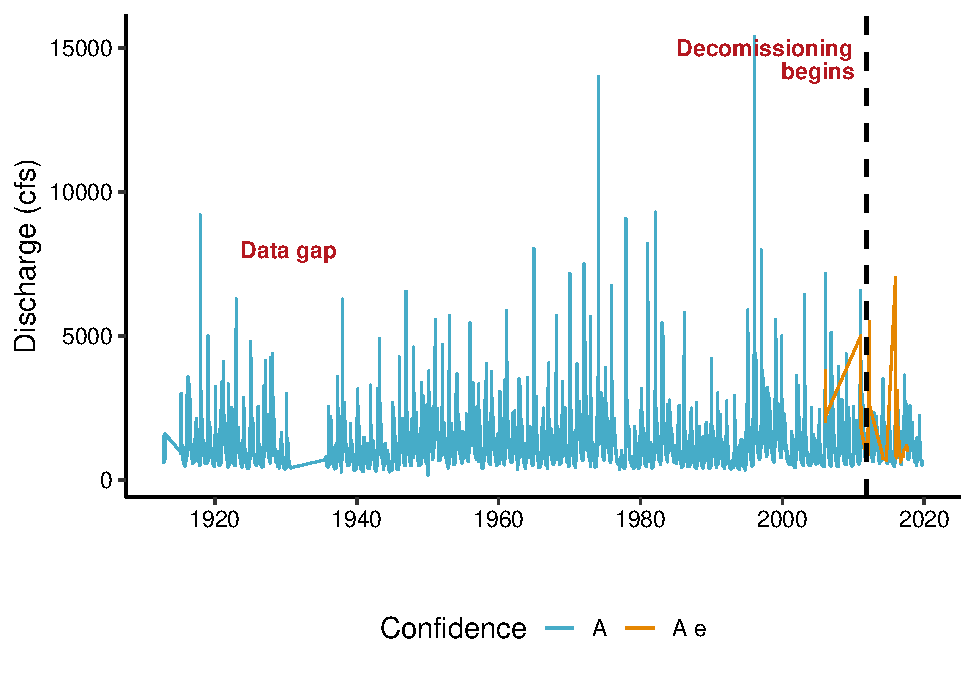
\includegraphics{WhiteSalmon_WriteUp_files/figure-latex/fig2-1.pdf}
\caption{Discharge over time with USGS QA/QC codes}
\end{figure}

\newpage

\begin{longtable}[]{@{}lrrrr@{}}
\caption{Descriptive statistics by period}\tabularnewline
\toprule
Statistics & p1940-2019 & p2003-2019 & p2003-2011 &
p2011-2019\tabularnewline
\midrule
\endfirsthead
\toprule
Statistics & p1940-2019 & p2003-2019 & p2003-2011 &
p2011-2019\tabularnewline
\midrule
\endhead
Min & 158.000 & 454.000 & 454.000 & 456.000\tabularnewline
10th percentile & 534.000 & 563.000 & 537.000 & 597.000\tabularnewline
25th percentile & 655.000 & 675.000 & 630.250 & 724.000\tabularnewline
Median & 936.000 & 956.000 & 917.000 & 986.000\tabularnewline
Mean & 1117.334 & 1102.946 & 1059.708 & 1146.332\tabularnewline
75th percentile & 1410.000 & 1360.000 & 1330.000 &
1430.000\tabularnewline
90th percentile & 1890.000 & 1830.000 & 1710.000 &
1950.000\tabularnewline
Max & 15400.000 & 7170.000 & 7170.000 & 7020.000\tabularnewline
\bottomrule
\end{longtable}

\begin{figure}
\centering
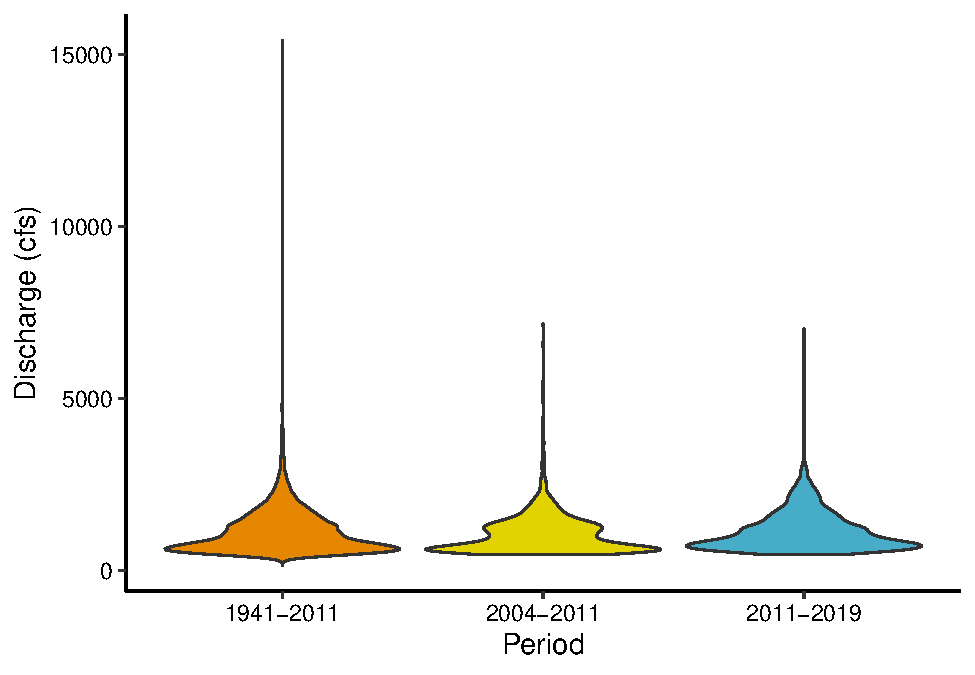
\includegraphics{WhiteSalmon_WriteUp_files/figure-latex/fig3-1.pdf}
\caption{Discharge during different periods on the White Salmon River.}
\end{figure}

\newpage

\begin{figure}
\centering
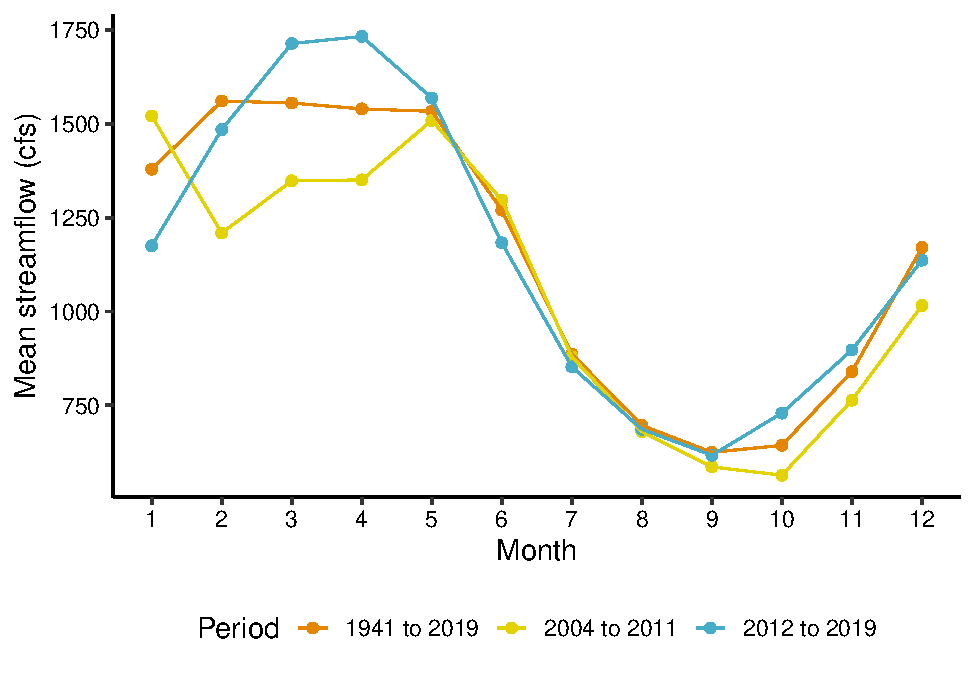
\includegraphics{WhiteSalmon_WriteUp_files/figure-latex/fig4-1.pdf}
\caption{Monthly averages by period.}
\end{figure}

\newpage

\hypertarget{analysis}{%
\section{Analysis}\label{analysis}}

\hypertarget{question-1-have-peak-flows-changed-since-the-condit-dam-was-removed}{%
\subsection{Question 1: Have peak flows changed since the Condit dam was
removed?}\label{question-1-have-peak-flows-changed-since-the-condit-dam-was-removed}}

Flood return intervals were modeled based on the period of record
discharge data (1941-2019). Return intervals for the 2004-2011 and
2012-2019 water years were then created to compare peak discharge
estimates for given intervals (100, 200, 500 and 1,000 year flood return
intervals). The 2004-2011 period was used to visualize pre-dam removal
conditions in the years leading up to the dam removal. The 2004-2011
period was included in order to visually assess if there were dramatic
differences in flood regimes in the years leading up to the dam removal.
The rationale for needing this visualization is that there could have
been either basin level land-use changes, precipitation changes, or,
most importantly, dam release changes that could have materialized in
recent years compared to the historic trends from the 1940s. Looking at
such a short period also removes peak events from the dataset. Given
that there were no major flood events from 2004-2019, the 2004-2019
visualization is almost functioning as a `reference condition' by which
to judge the 2011-2019 model (although given annual fluctuations in
precipitation, there is no true `reference condition').

Flood return intervals were created by parsing and ranking annual peak
flows from the datasets, followed by dividing the number of years by the
ranked peaks. The annual probability associated with these return
intervals was calculated. The logged return interval values were then
put into a linear model against the peak flows for each period. Using
these linear models, estimates for the 100, 200, 500 and 1,000 year
flood return intervals were calculated using the predict function. As a
reference, the 100 year flood return interval based on the period of
record is 14,386 cfs.

The results of these models show that estimated return intervals after
the Condit Dam was removed range from approximately 1,700 to 2,500 cfs
lower than the period of record estimates (Figure 5, Table 2).
Similarly, the return intervals after dam removal are range from
approximately 1,200 to 1,600 cfs lower than the 2004-2011 period
estimates. These results suggest that annual peak flows are lower now
that the Condit Dam has been removed. Recall in Figure 4 that monthly
averages during the rainy season appeared to be higher. This could
suggest that flows are more consistently high during the rainy seasons,
with less incidences of dam-release-related peaks. However, there are a
few major caveats here. The largest problem with this assessment is that
the linear model for the return intervals for 2004-2011 and 2011-2019
are based on only 8 sample points (annual peaks) each. This is reflected
in Table 2, which shows the combined period of 2004-2019 as having
overall much lower return intervals than the stand alone periods of
2004-2011 and 2012-2019. More years of data are needed in order to
adequately model for the changes in flood regimes, but for now, this is
an interesting glimpse into potential patterns.

\begin{figure}
\centering
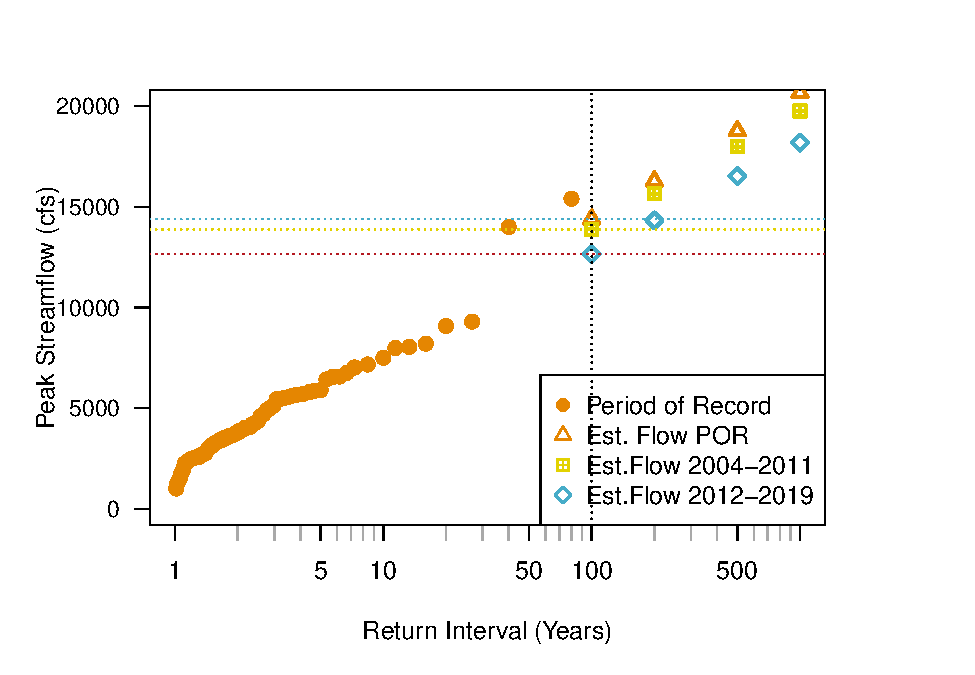
\includegraphics{WhiteSalmon_WriteUp_files/figure-latex/fig5-1.pdf}
\caption{Food return intervals modeled by period.}
\end{figure}

\begin{longtable}[]{@{}lrrrrr@{}}
\caption{Flood reutrn intervals modeled by period.}\tabularnewline
\toprule
Date Range & RI (100yr) & RI (500yr) & RI (1000yr) & No years & Adjusted
R2\tabularnewline
\midrule
\endfirsthead
\toprule
Date Range & RI (100yr) & RI (500yr) & RI (1000yr) & No years & Adjusted
R2\tabularnewline
\midrule
\endhead
1941-2019 & 14385.82 & 18767.23 & 20654.21 & 79 &
0.9649911\tabularnewline
2004-2019 & 11993.16 & 15479.37 & 16980.81 & 16 &
0.9394817\tabularnewline
2004-2011 & 13876.35 & 17991.03 & 19763.13 & 8 &
0.9379948\tabularnewline
2012-2019 & 12653.76 & 16524.85 & 18192.03 & 8 &
0.9561816\tabularnewline
\bottomrule
\end{longtable}

\hypertarget{question-2-have-low-flows-changed-since-the-condit-dam-was-removed}{%
\subsection{Question 2: Have low flows changed since the Condit dam was
removed?}\label{question-2-have-low-flows-changed-since-the-condit-dam-was-removed}}

The lowest 7-day average flow that occurred annually was calculated for
the period of record and the post-dam period. This is referred to as the
minimum Q7. The return intervals and annual probabilities were again
calculated from these parsed values. Unlike the flood return intervals,
in this case, the 7Q10 is the lowest 7-day average discharge that occurs
every 10 years. This 7Q10 value is a standard management metric for low
flows (EPA, 2018). The 7Q10 based on the period of record is 405 cfs,
whereas the 7Q10 for the 2012-2019 period is 452 cfs (Figure 6, Table
3). These calculations are once again based on linear models, in this
case using the minimum Q7 values against annual probabilities and then
using the predict function to find estimates for the annual probability
of exceeding the 7Q10.

For brevity sake, only the period of record and post dam removal period
were considered. The model shows that post dam removal low flows are
higher than the historic low flows, which when applied to point of
record daily discharge means, shows a substantial difference in number
of days of low flows (Figure 6, Table 3). This suggests that the natural
low flows in the White Salmon River below Condit Dam could have been
historically much higher prior to dam construction. The dam could have
been having significant ecological impacts that were simply not
perceived because the age of the structure predates the use of the 7Q10
for river management. Alternatively, again, the data being used to model
the 7Q10 since dam removal is limited. There is a need for more years of
data.

\begin{figure}
\centering
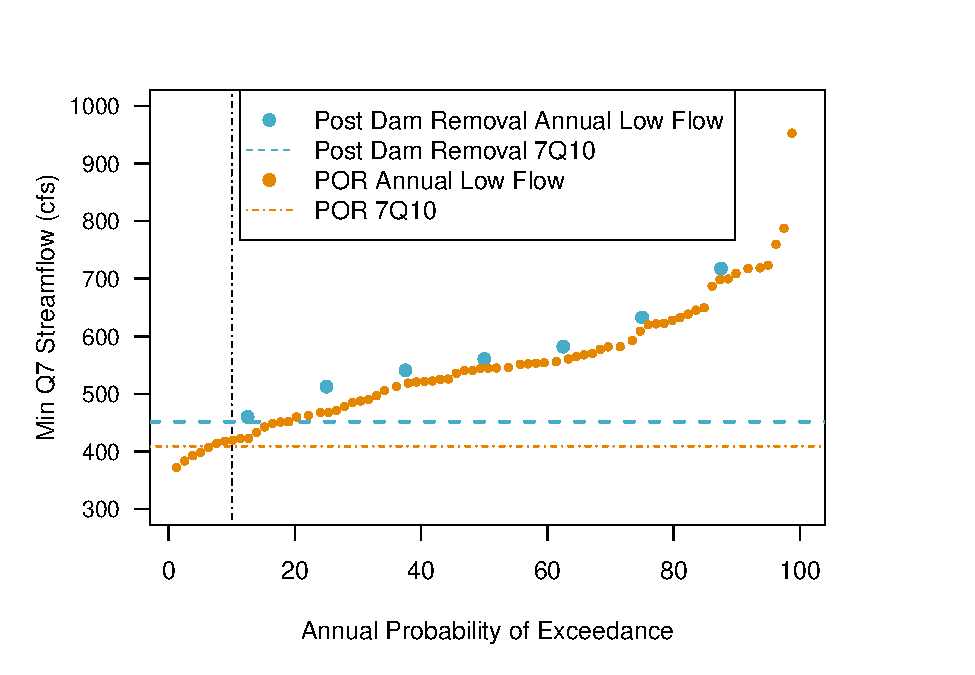
\includegraphics{WhiteSalmon_WriteUp_files/figure-latex/fig6-1.pdf}
\caption{Annual probability of exceeding the minimum Q7.}
\end{figure}

\begin{figure}
\centering
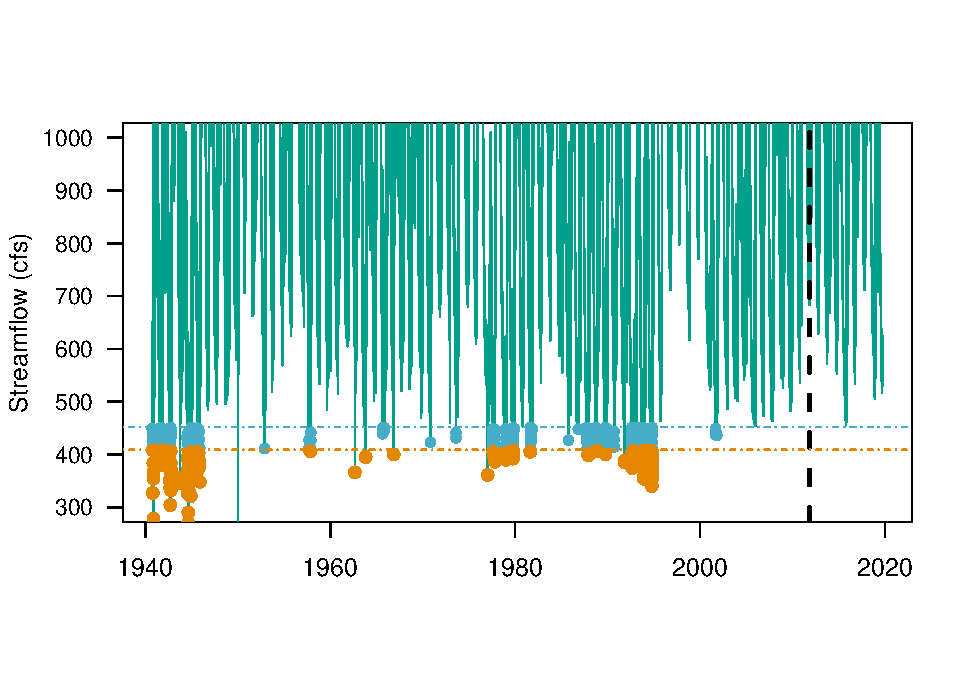
\includegraphics{WhiteSalmon_WriteUp_files/figure-latex/fig7-1.pdf}
\caption{The number of low flow days in the White Salmon River based on
the period of record and post dam removal period.}
\end{figure}

\begin{longtable}[]{@{}lrrrr@{}}
\caption{7Q10s on the White Salmon River. Note that the number of years
are the years where flows occur at or below 7Q10 within the entire
period of record based on the 7Q10 for the given period.}\tabularnewline
\toprule
Date Range & 7Q10 (cfs) & No Years & Annual Prob & Adjusted
R2\tabularnewline
\midrule
\endfirsthead
\toprule
Date Range & 7Q10 (cfs) & No Years & Annual Prob & Adjusted
R2\tabularnewline
\midrule
\endhead
1941-2019 & 408.85 & 21 & 26.25 & 0.89\tabularnewline
2012-2019 & 451.66 & 30 & 37.50 & 0.93\tabularnewline
\bottomrule
\end{longtable}

\hypertarget{question-3-is-there-a-significant-difference-between-historic-and-recent-conditions-and-post-dam-removal-conditions}{%
\subsection{Question 3: Is there a significant difference between
historic and recent conditions and post-dam removal
conditions?}\label{question-3-is-there-a-significant-difference-between-historic-and-recent-conditions-and-post-dam-removal-conditions}}

A Wilcox rank sum test was run on the historic and post-dam removal
datasets. A Welch's two sample t-test was run on the recent (2004-2011)
data and post-dam removal data. The choices to run these tests were
based on meeting assumptions associated with the compared datasets. The
Shapiro-Wilk normality tests all showed that these datasets do not have
normal distributions, as expected (p-values \textless{} 0.0001). An
F-test to compare two variances between historic and post dam removal
data showed the variances of the two datasets to be equal (F=1.41, df =
25931, p-value \textless{} 0.0001). This led to using the Wildox rank
sum test on these samples. The F-test to compare variances between
recent and post dam removal data showed the variances of the two
datasets to be unequal (F=1.02; df = 2921, p=value = 0.64).This led to
the use of Welch's t-test.

The results of these tests both showed the means and medians of the
compared samples to be significantly different (historic and post-dam
removal: Wilcox test, W = 35989876, p-value \textless{} 0.0001; recent
and post-dam removal: Welch's t-test, t =-5.78, p-value \textless{}
0.0001). Based on these tests, the discharge rates in the White Salmon
River are significantly different since the Condit Dam has been removed
- regardless of whether one looks at the historic data or the more
recent data (2004-2011) in comparison to post-dam removal conditions.
This is surprising given the violin plots in Figure 3, particularly for
the 2004-2011 and 2011-2019 periods which look very similar.

\hypertarget{question-4-are-seasonal-trends-becoming-more-or-less-monotonic-since-the-dam-was-removed}{%
\subsection{Question 4: Are seasonal trends becoming more or less
monotonic since the dam was
removed?}\label{question-4-are-seasonal-trends-becoming-more-or-less-monotonic-since-the-dam-was-removed}}

The Mann Kendall (MK) test is a non-parametric time series regression.
It does not require normal distribution, but it does require
independence of measurements. While it can be used with daily data, it
is more appropriately used, as done here, with monthly data to assure
that there is no serial correlation over time. Other assumptions for
Mann Kendall regressions include: true conditions, consistently
collected data (no gaps), and unbiased methods of measurement.
Therefore, it seems that all assumptions have been met for the MK tests.
The White Salmon was not expected to have significantly monotonic
trends; rather, the hypothesis here was that post dam conditions will be
less monotonic than pre-dam conditions. A higher p-value is used to
affirm this hypothesis. These tests were run on monthly data for two
time frames: 1966-2018 and 2004-2018. The results are broken up in two
ways: overall MK test results for given time period and seasonal
(monthly) MK test results for given time periods.

\hypertarget{overall-mk-test-results}{%
\subsubsection{Overall MK test results}\label{overall-mk-test-results}}

Seasonal discharge rates were historically monotonic, and even the time
period of 2004-2011 had significantly monotonic Seasonal discharge rates
(historic: z = -4.33, p-value \textless{} 0.0001, seasonal Sen's slope =
-1.46; recent pre-dam removal: z = 4.75, p-value \textless{} 0.0001,
seasonal Sen's slope = 41.60). Conversely, there are no significant
monotonic trends since the Condit dam was removed (post-dam removal: z =
-1.23, p-value = 0.218). Note that the Sen's slopes associated with
historic and 2004-2011 data show very different magnitudes of trends.
Historic data shows monotonic decrease in seasonal discharges of -1.46
cfs, whereas the 2004-2011 data shows a seasonal increase of 41.60 cfs
per year. The overall importance of these MK tests was to assess how
post-dam conditions have changed, and the one conclusion that can be
made is that monotonic trends have disappeared since the dam was
removed. There is a major caveat here that assessing seasonal trends on
an 8 year basis may not include enough data to provide reliable
statsitical results. The test results from these three different time
periods may be an artifice of this dilemma.The historic MK test results
are likely more dependable given the extent of the dataframe.

\hypertarget{seasonal-mk-test-results}{%
\subsubsection{Seasonal MK test
results}\label{seasonal-mk-test-results}}

The purpose of looking at MK test results for individual seasons was to
assess which seasons are seeing more/less monotonic trends based on the
p-values of these individual tests.Because the 2004-2011 data seems
potentially flawed due to its smaller sample size, I am only going to
look at the post-dam removal results compared to the historic
results.The results show that every month had less monotonic trends than
the historic data. Note that the post-dam removal resutls also come from
a smaller sample size; what these results signify are a glimpse of
trends so far. More years of data are needed for these tests to be
reliable. Even with the flaws in the datasets sizes, some additional
visualizations of monthly averages are included here with LOESS curves
in order to visualize the range in monthly values within these three
different datasets (Figures 8 and 9). These figures mimic the p-values
seen in the seasonal results, which overall show the ranges in discharge
to be more narrow in late summer to early fall and winter to spring
flows to have much higher ranges. In Figure 9, it appears that February
through July have experienced greater vacillation between low and high
monthly averages in discharge when compared annually. It is still early,
but this could be a sign that the dam was causing more monotonic flows
in the river through the storage of water during the rainy/wet season.
More years of data will be needed to assess the impact of dam removal.

There is a more complex story than expected when individual seasons for
these MK test results are reviewed. The historic data showed significant
monotonic trends for the months of September (S = -385, p-value = 0.06)
and October (S = -439, p-value = 0.03) - late fall before the rainy
season begins. The 2004-2011 data showed near significant monotonic
trends for the months of May (S = 15, p-value = 0.06) and June (S =16,
p-value = 0.06) - the beginning of the dry season. The historic data,
again, is more reliable given the dataset's size. That September and
October saw annual decreases in seasonal discharge rates suggests
potentially drier conditions later into winter. This could be caused by
climate change, or alternatively, it could be the result of dam
management practices shifting over time. Practices that could have
shifted include: drawing down the reservoir behind Condit dam earlier in
the season in order to make room for a higher volume of winter flows
(thus preventing infrastructure damage from high flows), or holding
water back later in fall due to a lack of precipitation (thus allowing
the dam to continue to produce electricity until the rainy season
begins). Assessing this trend would require modeling precipitation
trends within the basin.

\begin{figure}
\centering
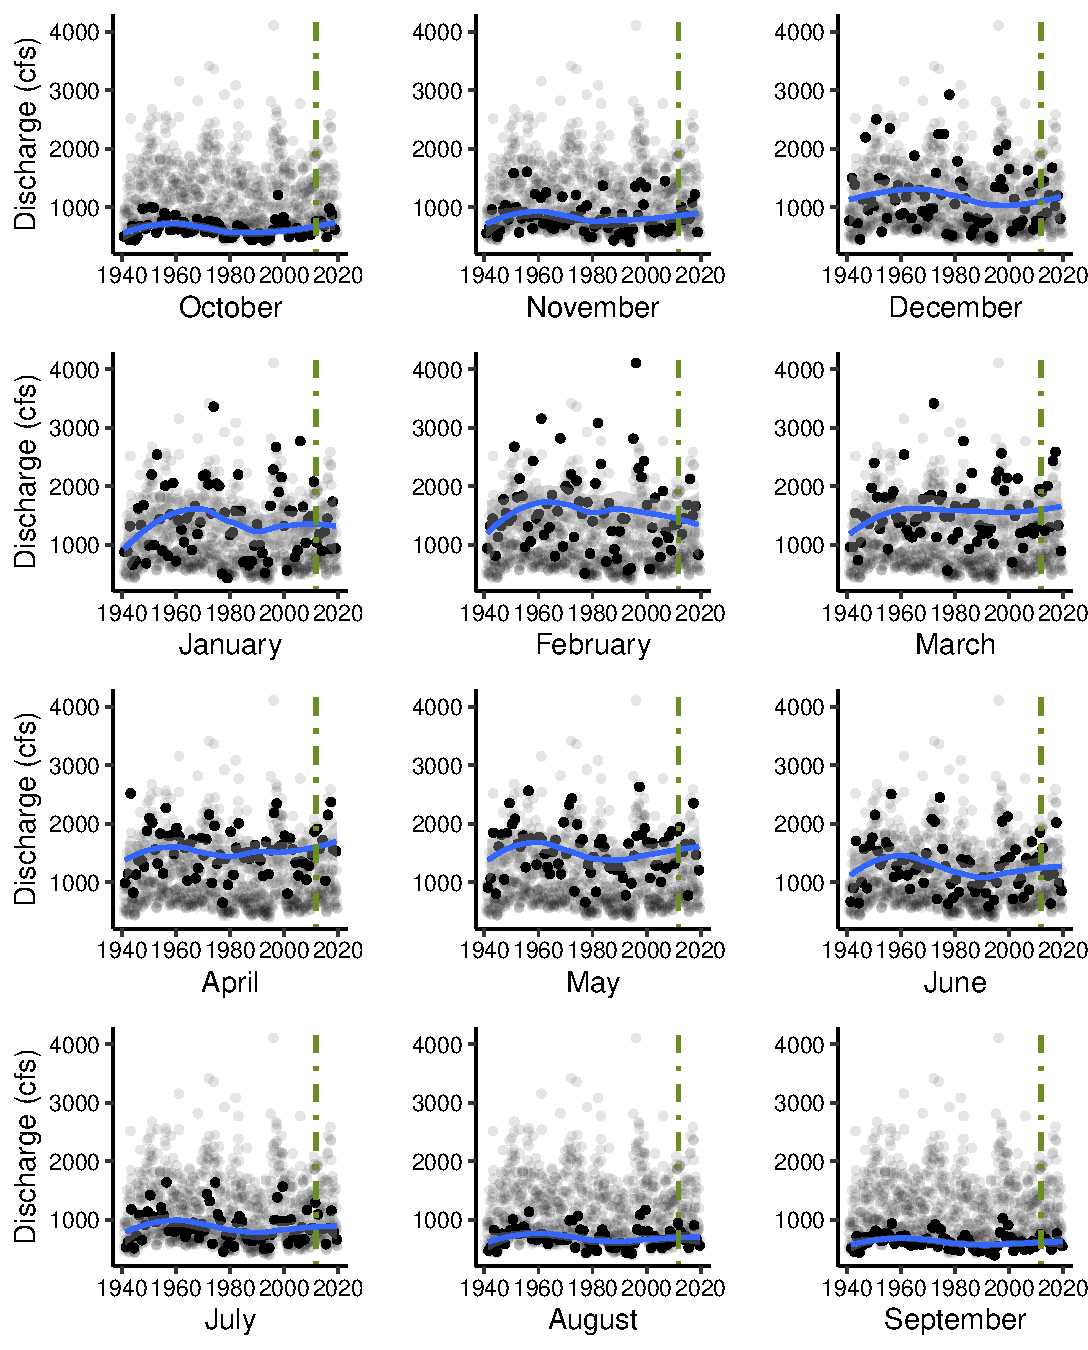
\includegraphics{WhiteSalmon_WriteUp_files/figure-latex/fig8-1.pdf}
\caption{Monthly LOESS curve fit to historic data (1941-2019 water
years) on the White Salmon River. Vertical dashed line signifies Condit
Dam removal.}
\end{figure}

\begin{figure}
\centering
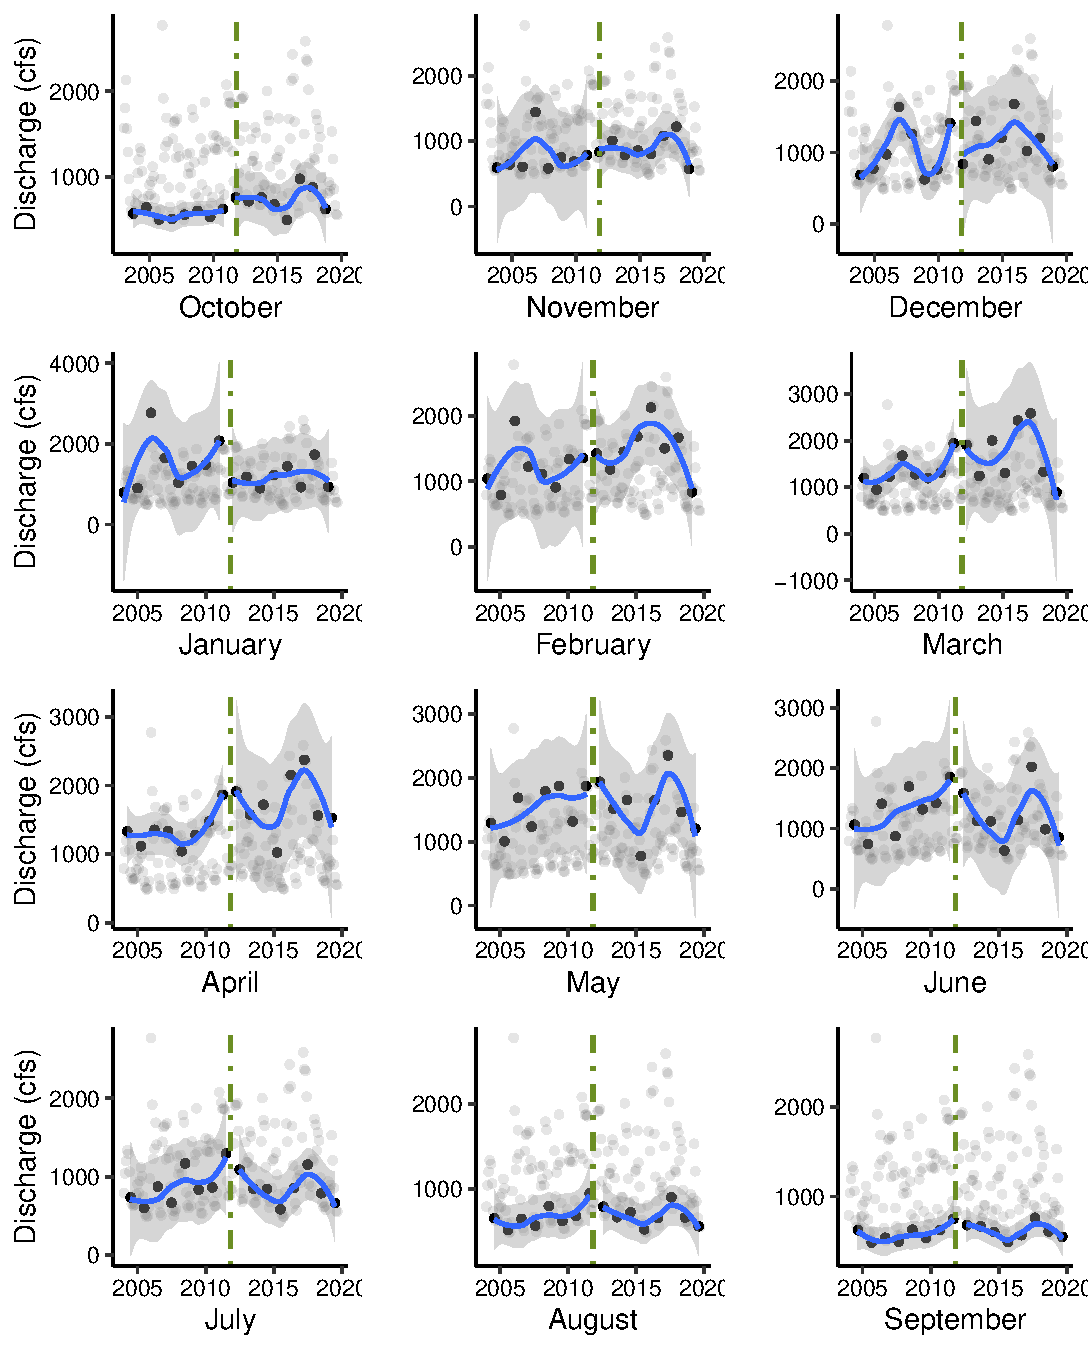
\includegraphics{WhiteSalmon_WriteUp_files/figure-latex/fig9-1.pdf}
\caption{Monthly LOESS curve fit to 2004-2011 and 2012-2019 water years
on the White Salmon River. Vertical dashed line signifies Condit Dam
removal.}
\end{figure}

\newpage

\hypertarget{summary-and-conclusions}{%
\section{Summary and Conclusions}\label{summary-and-conclusions}}

\newpage

\hypertarget{references}{%
\section{References}\label{references}}

\textless add references here if relevant, otherwise delete this
section\textgreater{}

\end{document}
